\RequirePackage[l2tabu, orthodox]{nag}
\documentclass[]{report}
\usepackage[utf8]{inputenc}

\usepackage[affil-it]{authblk}
\usepackage{etoolbox}
\usepackage{lmodern}
\usepackage[a4paper]{geometry}
\usepackage{graphicx}
\usepackage{microtype}
\usepackage{csquotes}
\usepackage{wrapfig}
\usepackage[british]{babel}
\usepackage[backend=biber,style=numeric]{biblatex}
\usepackage{alltt}
\usepackage[scaled=.90]{helvet}% Helvetica, served as a model for arial
\usepackage{caption}
\usepackage{subcaption}
\usepackage[colorinlistoftodos,prependcaption,textsize=tiny]{todonotes}
\usepackage{perpage}
\MakePerPage{footnote}
\usepackage{minted}

% hyperref loaded at end, only cleverref loaded after
\usepackage{hyperref}
\usepackage{xcolor}
\hypersetup{linkbordercolor=black,pdfborderstyle={/S/U/W 1},pageanchor=false}
\usepackage{cleveref} % use \cref to make references

\patchcmd{\abstract}{\titlepage}{}{}{}
\patchcmd{\endabstract}{\endtitlepage}{}{}

\providecommand{\tightlist}{%
  \setlength{\itemsep}{0pt}\setlength{\parskip}{0pt}}

\renewcommand{\thefootnote}{\roman{footnote}}


% problem env
\newcounter{problemctr}
\newenvironment{problem}[1][]{%      define a custom environment
  \refstepcounter{problemctr}% increment the environment's counter

  \addcontentsline{toc}{subsection}{Problem \arabic{problemctr}}%
  \bigskip\noindent%         create a vertical offset to previous material

  \noindent
  \textbf{Problem \arabic{problemctr} #1}% or \textbf, \textit, ...
  \newline%
  \newline%
  \noindent
}{\par\bigskip}%          create a vertical offset to following material


% requirement env
\newcounter{requirementctr}
\newenvironment{requirement}[1][]{%      define a custom environment
  \refstepcounter{requirementctr}% increment the environment's counter

  \addcontentsline{toc}{subsection}{Requirement \arabic{requirementctr}}%
  \bigskip\noindent%         create a vertical offset to previous material

  \noindent
  \textbf{Requirement \arabic{requirementctr} \textit{#1}}% or \textbf, \textit, ...
  \newline%
  \newline%
  \noindent
}{\par\bigskip}%          create a vertical offset to following material


% usecase env
\newcounter{usecasectr}
\newenvironment{usecase}[1][]{%      define a custom environment
  \refstepcounter{usecasectr}% increment the environment's counter

  \addcontentsline{toc}{subsection}{Use-Case \arabic{usecasectr}}%
  \bigskip\noindent%         create a vertical offset to previous material

  \noindent
  \textbf{Use-Case \arabic{usecasectr} #1}% or \textbf, \textit, ...
  \newline%
  \newline%
  \noindent
}{\par\bigskip}%          create a vertical offset to following material



\addbibresource{bibliography.bib}

\begin{document}


\begin{titlepage}
  \normalfont\sffamily  
	\centering
	
\includegraphics[width=0.6\textwidth]{Figures/UniOfManchesterLogo.eps}\par\vspace{1cm}
	%{\scshape\LARGE The University of Manchester \par}
	\vspace{1cm}
	{\scshape\Large Third year project\par}
	\vspace{1.5cm}
	{\huge\bfseries A Notebook-Style SQL IDE\par}
	\vspace{2cm}
	{\Large\itshape James Peach\par}
	\vfill
	supervised by\par
	Alvaro. A. A. \textsc{Fernandes}

	\vfill

% Bottom of the page
	{\large \today\par}
\end{titlepage}

\begin{titlepage}

\begin{abstract}
  
   Developers require an understanding of the task at hand in order to do their job. 
   Sometimes this information comes from documentation, other times it comes from
   code and comments. Having separated code and documentation means developers have to
   read and update two sets of information.
   This duplication of effort can lead to mistakes especially when switching between 
   code and notes. The goal of the project is to create a tool in which both the code and the 
   documentation can coexist and solve some of the problems that can occur when 
   using existing solutions.

\end{abstract}

\renewcommand{\abstractname}{Acknowledgements}

\begin{abstract}

    This project was developed at the University of Manchester, I would like
    to thank my tutor Alvaro for his help and support throughout all of
    these years and for his patience through the lengthy discussions on
    those occasions where my understanding needed expanding.

    Thanks also goes to my patient editors, my dad Anthony and my friend George.
  
\end{abstract}

\end{titlepage}
\tableofcontents


\chapter{Introduction}\label{introduction}

Developers use documentation to aid their understanding of code, however the
documentation is often constructed and viewed on paper or in a web browser. An
example for Java applications is \textit{Javadoc}\cite{javadoc}. While the use
of a documentation tools provides a good overview of the code, it shouldn't
exist in isolation.  Developers can't rely on the documentation alone, they must
also have an understanding of the other components of the system and their
interaction.

This is also true of database applications. Database applications are often the
backing store for the data of the system and also provide a center for the
business logic for the application. They are often at the center of large
applications and as a result they can be complicated. This is because databases
are designed to store and validate large amounts of data. They also provide many
useful mechanisms for integrating with a large number of other technologies.

It is therefore important that the developers that develop and manage
these applications know exactly the effects of the code and what there
changes mean in terms of the system as a whole.

\section{Goal}\label{project-goal}

The project's goals are to create an application that will help database
developers to document and code in a more consistent and interactive
manner. The result should try to accomplish this within one tool, both for coding, and for documenting.

The project will cover methods for identifying the problems with existing
applications, and formalizing them. The project then aims to provide an
evaluation of the different approaches to solving the problems along with
reasons for any choices made.

\section{Users}\label{users}

In order to understand the application we first need to understand the
users of the application. These users are developers. The developer's
days could consist of many different types of tasks, including developing new
applications, new features, and maintaining old applications and
services. These are just a few of the most common tasks required.

This poses problems when creating software for these developers to use; while
they require places to document code and other items, they do not do so with a
common structure. The tools they use must support their individual ways of
working. However they do still need ways of helping them to manage the
information.

Creating an application for this purpose will require considering the many
problems that existing applications have attempted to tackle and their success.

One example of the type of problems an organization application would look to
solve is this: A developer is working on more than one application and is
responsible for supporting older applications. The developer receives notice
that a problem exists with a project he worked on previously. His current
progress needs to be noted so he can continue at a later date. The developer
then must find details about the problem. The process of switching projects and
finding the required information is a problem this project aims to solve.

The problem above is just one problem and there are many more that would need to
be identified. This report details how they were found and their solutions
designed and built.

\section{Overview of the report}\label{overview-of-the-report}

This report explains how the final solution was developed from an idea
into the final product. It does so with some guidance from standard
software development techniques. First, some problems are identified, then
a formal set of requirements is derived. These requirements guide the
design of the application and after the application is built the
requirements are again used to verify that the end product does indeed
solve the original problems identified.

The problems that the application hopes to address will be a collection
of things that occur in every day life as a developer and other problems
identified with existing tools available.

\chapter{Background}\label{background}

In this chapter the reason for a documentation tool is outlined and some
existing solutions are described. Each existing solution will be analysed for
its strengths and weaknesses.

If code is written without comments or detail about what is to be
achieved, it is possible that when the code is read again in the future, the
original intent will have been lost. The decisions the developer made about the implemented
solution have been lost.

There are many different ways to document code ranging from
completely offline to completely digital and many different methods for
integrating code. The most simple offline approaches consist of simple
notepad pages with notes and diagrams. This offers a totally free-form
approach to note taking as with pen and paper there is no limit to what
you can make notes about. Tables diagrams and hand written pseudo code
can be easily drawn and annotated. While this is suitable for some
circumstances it isn't for others. For example if you had an email you wanted
to include in your notes it would have to be printed and filed in the notes.
This leads to problems of printing and loosing the loose pages.

One solution for this problem is the many solutions for electronic or digital
notes. \textit{Evernote}\cite{evernote}, is a popular choice for notes and offers
a wide range of platforms for note creation however it is not designed with code
documentation specifically in mind. While it is a very good solution for taking
notes, as is evident in the number of users\footnote{The current ranking of
Evernote by Alexa is 397
\href{http://www.alexa.com/siteinfo/evernote.com}{http://www.alexa.com/siteinfo/evernote.com}}.
the lack of specific features aimed at developers e.g. version control makes it
difficult to use for documentation.

The above solutions are not tailored to suit the specific task of making notes
for SQL developers. Tools used by developers can both develop new code and help
document it for future readers. Commenting code is often the closest notes get
to the code. Well commented code can help developers to both remember the code
they wrote in the past and understand new code. Comments provide an excellent
opportunity to pass details of previous attempts from programmer to programmer.

Comments on code can often not last the test of time as they don't force you to
update your note when the code they refer to changes. For example, over time the
commented function might offer more options or deviate from its original
purpose. Unless the developer remembers to update the comment then, over time, this could lead to confusion.

\section{Analysis of existing solutions}\label{analysis-of-existing-solutions}

The different applications vary with programming language and
operating system. They each have positives and negatives.

Each is analysed below with a brief overview of the functionality provided and
details on specific positives and negatives. After the analysis of the existing
solutions the problems will be summarised before requirements are set out.


\begin{figure}
  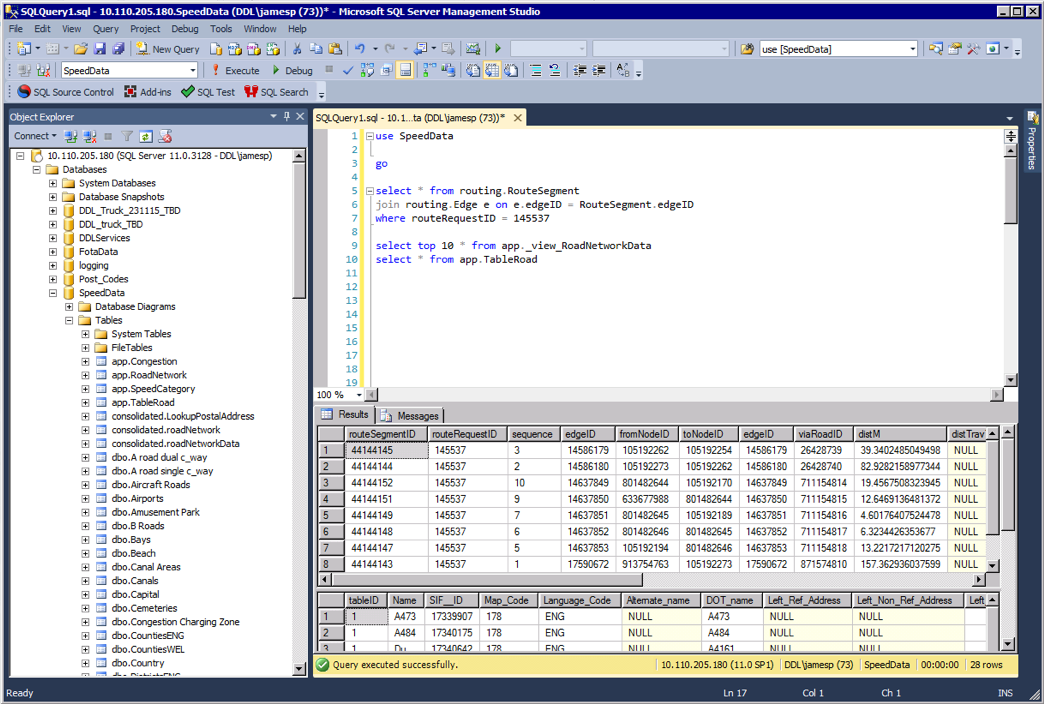
\includegraphics[width=\linewidth]{Figures/SSMS.png}
  \caption{SQL Server Management Studio, Microsoft: Main workspace with open queries and results}
  \label{fig:ssms}
\end{figure}

\subsection{Microsoft SQL Server Management Studio}\label{microsoft-sql-server-management-studio}

\noindent
See fig \ref{fig:ssms} for a screenshot.

\noindent

\textbf{Product URL}\cite{ssms}
\url{https://msdn.microsoft.com/en-us/library/hh213248.aspx}



An official offering for the Microsoft SQL Server Database server. The ability
to open multiple connections to databases and have many open files in an IDE
powered with the Microsoft Visual Studio Shell\cite{vsshell}. The application
offers no management of files within the tool, it does however, offer the
ability to open files from the filesystem. The tool allows for the execution of
queries and the result viewing pane shows a table containing the output. The
results in the result pane can not be stored in the application or with the
query for later review. If this is a requirement of a user it must be done
manually with the export function.

As with many database servers the functions and procedures are stored within the
databases and so any files on the local system might not be in sync with the
ones on the server. The application is a native windows application and offers
no alternatives for other operating systems. Developers have the ability to
connect via TCP, Shared memory, and named pipes. This allows for connections to
be made from anywhere with a suitably open internet connection however it poses
many problems when on a restricted network and limits users to use Microsoft's
own operating system as the application is for Windows only.

\blockquote{Windows 10, Windows 8, Windows 8.1, Windows 7 (SP1), Windows Server 2012 (64-bit), Windows Server 2012 R2 (64-bit), Windows Server 2008 R2 (64-bit)}

From SSMS 2016 preview download page \cite{ssmsdownload}.


\begin{figure}
  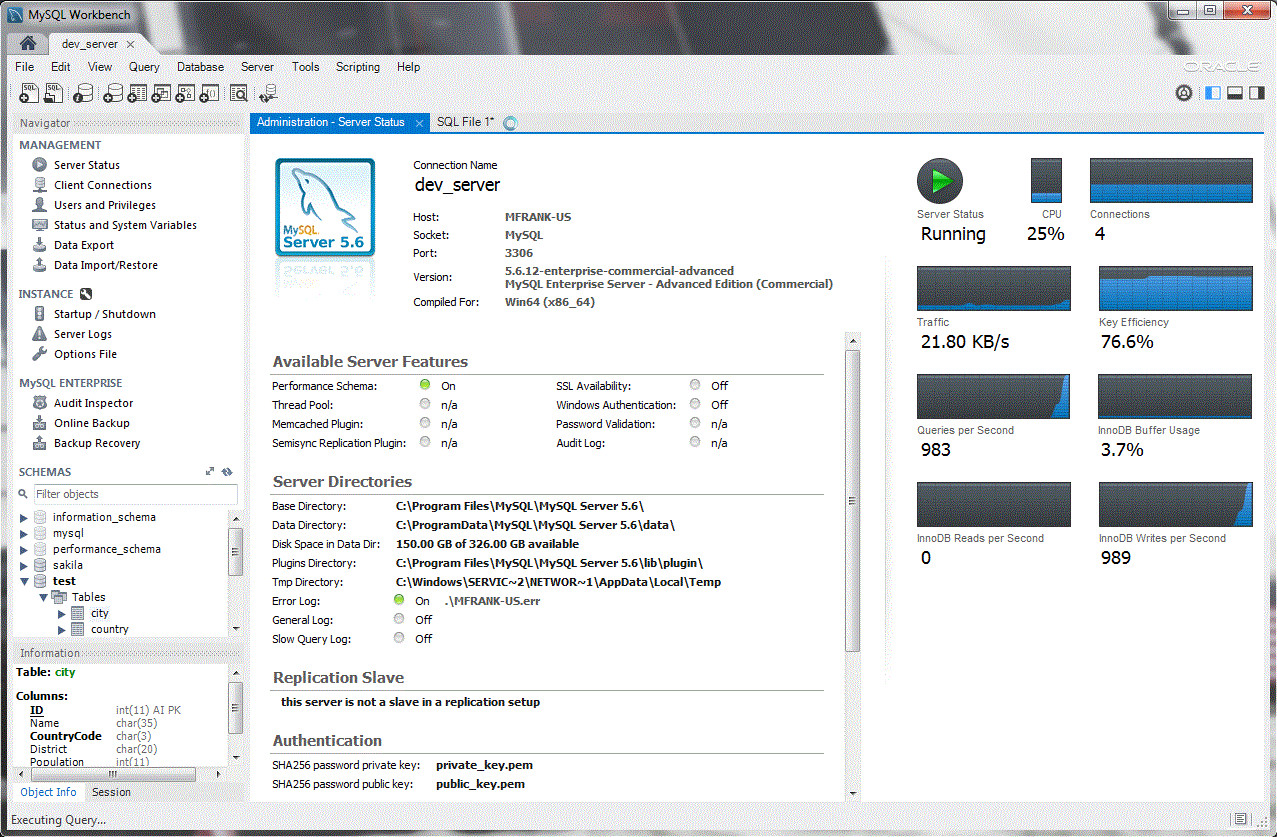
\includegraphics[width=\linewidth]{Figures/MySqlWorkbench.png}
  \caption{MySql Workbench, Oracle: Home screen}
  \label{fig:mysqlworkbench}
\end{figure}

\subsection{MySQL Workbench}\label{mysql-workbench}

\noindent
See fig \ref{fig:mysqlworkbench} for a screenshot.

\noindent
\textbf{Product URL}\cite{mysqlworkbench}
\url{https://www.mysql.com/products/workbench/}


The MySQL Workbench offers a multi-platform solution for accessing a MySql
database. The tool also offers a model management tool (fig
\ref{fig:mysqlworkbenchmodel}) for designing a logical model of the database
entities and relations. This provides a way to easily view a high level
overview and make useful annotations that go above and beyond simple comments
written separately. For more information Oracle have published a paper
detailing the creation of the tool\cite{mysqlworkbenchmodeldesign}.

\begin{figure}
  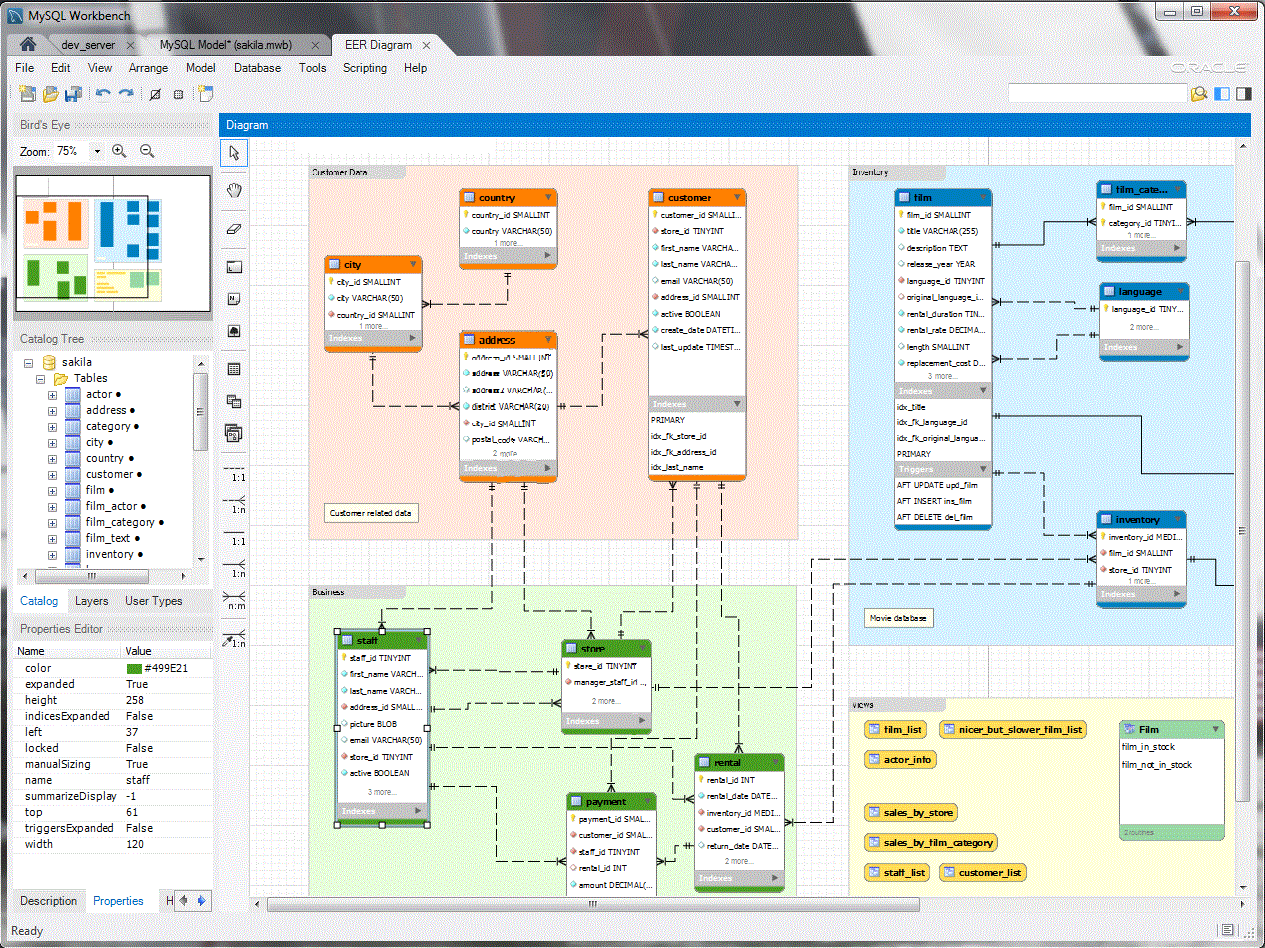
\includegraphics[width=\linewidth]{Figures/MySqlWorkbenchModel.png}
  \caption{MySql Workbench, Oracle: Visual Database Design feature}
  \label{fig:mysqlworkbenchmodel}
\end{figure}

The Workbench also offers multi-platform capability. Providing more ways for the
users of an application to access it, this helps integrate a tool into the 
workflow of the developer. Having to switch between operating systems when your database
management software is not available on the same operating system as your application
development environment can be very disruptive to a development workflow. The
development of this project should aim to support common platforms.


\begin{figure}
  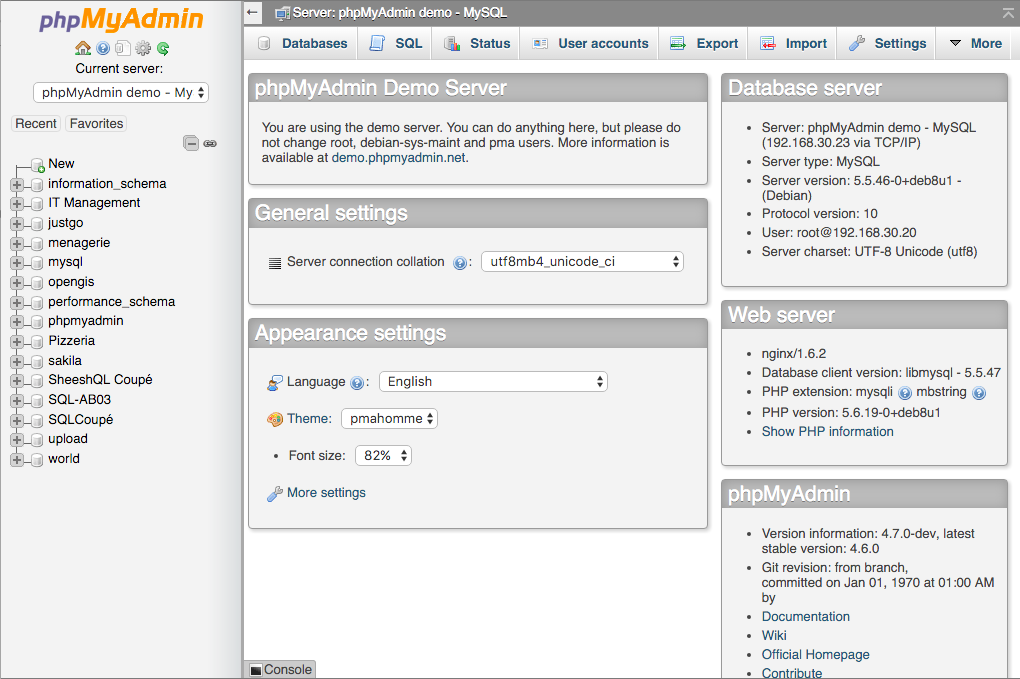
\includegraphics[width=\linewidth]{Figures/phpmyadmin.png}
  \caption{phpMyAdmin: home page}
  \label{fig:phpmyadmin}
\end{figure}


\subsection{phpMyAdmin}\label{phpmyadmin}

\noindent
See fig \ref{fig:phpmyadmin} for a screenshot.

\noindent
\textbf{Product URL}\cite{phpmyadmin}
\url{https://www.phpmyadmin.net/}


The alternative to the official MySqlWorkbench is an open source web
based solution for easy access to the database from anywhere you have an
internet connection. phpMyAdmin is a PHP web application and needs a
hosting server to provide access. The application, once running
has a secure login system with the ability to view and edit data in the
system.

However the tool offers little in the way of editing for scripts and
database code. Bulk manipulation of data is not offered in the
application but instead through the export of multiple different file
types.

The application also analyses the foreign keys in the database and provides access to the referenced rows in the related tables. This feature can make viewing the data in the system more intuitive as related data need not be separately queried for.

Unlike the MySql Workbench there is no designer for models and all
changes are done to the database ``live'' there is no design and publish
as offered in MySql workbench.


\begin{figure}
  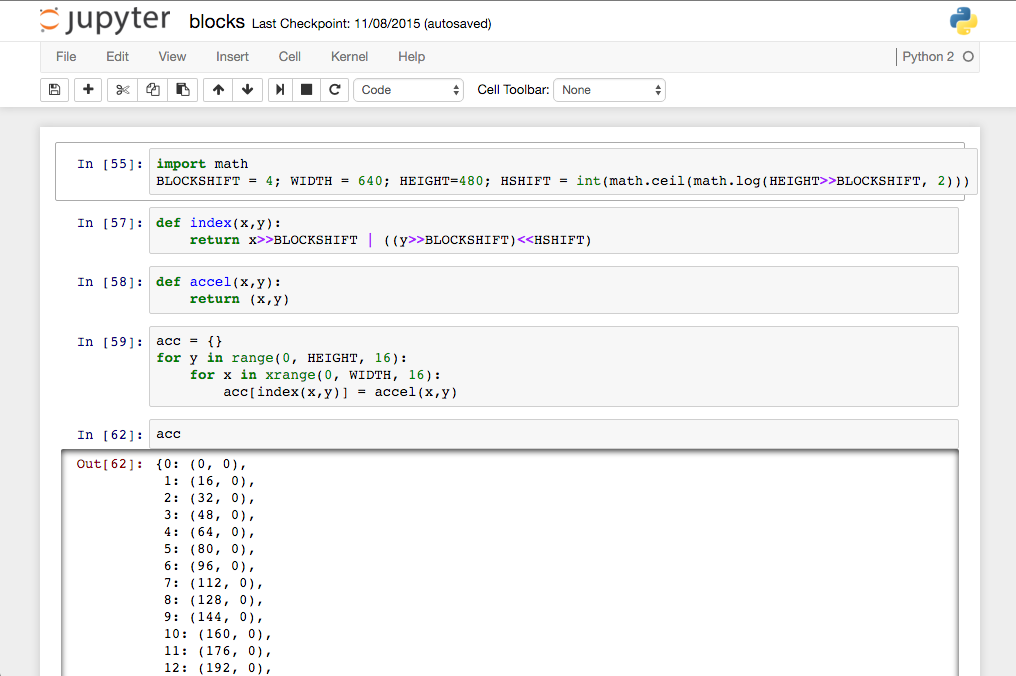
\includegraphics[width=\linewidth]{Figures/ipython.png}
  \caption{IPython Notebook, example notebook}
  \label{fig:ipythonnotebook}
\end{figure}

\subsection{IPython / Jupyter}\label{ipython-jupyter}

\noindent
See fig \ref{fig:ipythonnotebook} for a screenshot.

\noindent
\textbf{Product URL}\cite{PER-GRA:2007}
\url{http://ipython.org/}

IPython, now Jupyter, differs from other solutions evaluated above as it is not
a SQL IDE as such it doesn't show any specific features for SQL code in
particular, however, the integration between the code and the text in the editor
is done in a very easy to use way.

IPython provides an interactive browser based coding tool, the ``notebook''. The
notebook provides the ability to create cells for code and text. These code cells
can then be executed and results are shown below the code. This provides a
visual relationship between the code and its output. The text cells are
formatted with Markdown\cite{wiki:markdown}.

\begin{figure}
  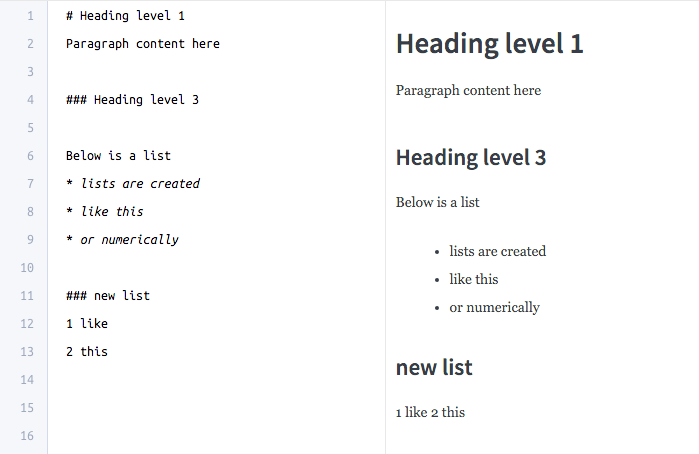
\includegraphics[width=\linewidth]{Figures/markdown.png}
  \caption{Markdown: example markdown source (left) and output (right)}
  \label{fig:markdownexample}
\end{figure}

Markdown (fig \ref{fig:markdownexample}) is a simple written markup language for
textual documents. Markdown provides simple ways to create headings and lists
paragraphs while balancing this with simple easy to read minimal formatting.

The mix of executable code within the text notes provides a unique
experience. The ability to see and tweak code and have a well
presented explanation of the code.

Interactive code and results as done in an IPython notebook provide a
quick way to see the results of the code. This allows and promotes the
testing and exploration of the code and can help the developer to
understand exactly what effects each part of the code has on the end
result. This is important because developers who understand the impact of the
existing code and their changes to it will create fewer bugs in code and are
more productive.

The notebooks reside on files on the local disk of the system, much like
any other file. As such the organisation of the files is left up to you
the creator to file them in folders etc. This can be a problem for long term
users of the application as while the individual files might be organised, if
the collection of files is haphazard then the organisation problem has just
moved to another part of the process.

\section{Problems}\label{problems}

\begin{problem}{Keeping notes of important things}

As developers work on their projects and as these projects evolve there
becomes an increasing number of things that need to be understood in
order to develop / maintain the project. The problem is to provide an
easy flexible way to make notes on different topics and allow access to
the notes in an organised way.

\end{problem}

\begin{problem}{Notes are only useful when they are read}

The notes / code stored need to be accessible for developers, they are read
more times than they are modified. This shows the importance of the time spent
documenting the code when it is first written.

The notes as discussed do not have an implicit structure and so a helpful
search is difficult to create. Most solutions just offer full text
search of the data.

The notes might have had several revisions over time and might need the
information accessible from the past.

\end{problem}


\begin{problem}{Notes that include code are often not
updated}

The notes, in some note taking applications that store code, are often not in an
executable format. This code will have dependencies as code does not exist in
isolation. For example the functions used or the tables referenced may be
modified. If the code in the note can not be directly executed, these changed
in the context can create bugs in the code that wont be immediately visible and
could mislead the reader.

This is a problem because the code is only useful in a note when it is
up to date and bug free, often at the time of writing it is correct but
as the system changes the code can become out of date.

The problem is how to ensure or help the user to keep this code up to
date within the note.

\end{problem}

\begin{problem}{Data always changing}

The data in database systems is always changing. When the system was
written the data might have looked significantly different to what it is
now. This makes things hard to compare as time goes on.

The problem is how to ensure that, even if the underlying data is
changed, the note and code within is still useful for other developers
in the future.

\end{problem}

\begin{problem}{System access}

Developers need easy access to the information and the database from in or out
of the office. Current solutions for IDE's are often system specific and
don't offer good cross platform compatibility.

The problem is providing access to the data and system from whatever
system, and wherever the developer is in a secure way.
\end{problem}

\begin{problem}{Cross referencing}

When writing documents, often it is required to provide context. This is done
by referring to other parts of the same or different document. Providing a
solution to this problem will benefit both the readers and writers and help
communicate the information.

\end{problem}

\section{Problem summary}\label{summary-of-identified-problems}

The problems identified above fall into different categories:

\begin{itemize}
\tightlist
\item
  Organisation of notes
\item
  SQL specific problems
\item
  Searching notes
\end{itemize}

Each of the above categories of problems could be tackled in many different
ways. The next stage in the development of a complete solution is to identify
some concrete requirements and use cases for the application and discuss the
different approaches available. Each approach has downsides, these need to be
properly analysed and evaluated to provide a solution.

\chapter{Requirements}\label{requirements}

The existing solutions have provided a basis for identifying the
potential problems the system must overcome. Along with other sources
and other base requirements a set of more formal requirements are listed
below.
\section{Requirements}

The requirements will be detailed below, along with a brief reason for the
importance.

\begin{requirement}
The application must store notes about the project in various separate
``files'' within the system. The files can take on any form however it is
required that they are separate entities.

The files must exist in separate items so that each can have a well defined
topic. This will aid the user in placing notes in the correct locations.
\end{requirement}

\begin{requirement}
The ``files'' stored within the system must be able to store code and also
notes in a format easily read.

For example these files should have the ability to contain syntax highlighted
code and also headings lists.
\end{requirement}

\begin{requirement}\label{requirement:accessible}
The application should be easily accessible from multiple operating systems.

The targeted operating systems should include Windows, Popular flavors of
linux, and Mac OSX.
\end{requirement}

\begin{requirement}
The application should have the ability to view the results of queries executed
on the system in table form.

This is the de-facto representation of the results from a SQL query, although
it may be possible to view the results as plain text, the requirement is to
display them in tabular form.
\end{requirement}

\begin{requirement}{(Optional)}
The ability to detect the type of result and view it in a
more suitable form. The more suitable form could be anything from a
graph to folder structure to a specific viewer for xml documents.

This could be implemented in a way that automatically selects the best result
format for the results. However, this could also be completed with a manual
selection of the result type that changes the display format.
\end{requirement}

\begin{requirement}
The application should have a mechanism for organizing related files in
a hierarchy. Files that are about a part of the system should be stored
in the same place in the system.

This requirement is non specific so as to not restrict the choice of possible
implementations. The need to organize files is an old requirement. Many
existing systems both specifically related to code and in general have
mechanisms in place for this.
\end{requirement}

\begin{requirement}
The application should save the previous versions of the files stored within.
These versions should allow editing and saving over newer versions if needed.

Developers often have to revise code and often new features are added to
existing systems. The ability to see previous versions of code is necessary in
order to provide adequate context to developers.
\end{requirement}

\begin{requirement}
The application should allow for multiple files to
be open at once and viewed at the same time. This can be done in a free
sized window mode or windows listed vertically or horizontally.

The ability to work on multiple files at the same time will help the developer
to remember the details of the different tasks without the possibility to
forget one entirely.
\end{requirement}

\begin{requirement}
The application should allow for searching for strings in files.

When searching through documents the ability to find a single occurrence of a
word or phrase in many documents can drastically decrease the time needed to
continue working. When trying to complete an action, the time taken to find a
file needed, determines the chance of forgetting the task.
\end{requirement}

\begin{requirement}{(Optional)}
The ability to view, in each of the search results, where the search phrase was
found. And the ability to open the file from the search result.

When searching, the context around the match is often very important and can
help identify the right instance of the phrase. Because when searching, in most
cases the searcher is only interested in one location of the phrase.
\end{requirement}

\begin{requirement}
The application should allow for the easy comparison results. Historic results
of the queries should be shown as a diff or side by side with newly executed
results.

Within the database, the data can change frequently. The ability to save
previous versions of the results of the queries and then compare them with new
versions can have many different uses. For example a query might not be as
performant as required. The developer will need some method to verify that the
results from before the changes is the same as the optimized version.
\end{requirement}

\section{Use cases of the system}\label{use-cases-of-the-system}

The use cases of the system will detail how the system is intended to be used.
The specific and important use cases will give context to the requirements.

The primary users of the system as discussed are the developers of the projects
themselves. The uses will be performing some tasks more than others and some
will have more of an impact on the use of the application than others. The
important use cases are captured below to aid development and evaluation.

\begin{usecase}
Developer wishes to document information about a development.

The correct file must be found in an existing project and amended with details
of the new development.
\end{usecase}
\begin{usecase}
Developer needs to view all documents pertaining to a project in the
system.

The collection of files for a project must be identified within the
application.
\end{usecase}
\begin{usecase}
Developer needs to find reference to a particular item within the system
but is unfamiliar with the specific location or other detail

\end{usecase}
\begin{usecase}
Developer has to find specific details of a system previously worked on
in order to maintain it.

\end{usecase}
\begin{usecase}
Developer wants to view and compare previous versions of some code
within the database

\end{usecase}
\begin{usecase}
Developer want to view the versions of files within the notebook.

The different states of a piece of code (query) in the system need to be identified and the saved results compared.

\end{usecase}
\begin{usecase}
The developer wants to find the places a particular entity is used
within the system to better understand how the changes planned could
effect the system as a whole. \footnote{%
  This is known as %
  \href{https://en.wikipedia.org/wiki/Change\_impact\_analysis}{impact
analysis}%
}

\end{usecase}

\subsection{Priority of requirements}

Some of the above requirements and use cases are more important than others. For example providing a method for finding files in the system will have to come after the ability to create files.
The priority of the requirements and use cases will be determined in the development process.

\chapter{Design}\label{design}

The design of the application will draw from the above requirements and
the associated use cases to form a final application. There are many
decisions to be made when designing an application, each decision needs to be solved in the best way possible given the conditions and the available solutions and development time.

In this chapter some design problems are listed and a discussion is provided for each on a selection of solutions. Each candidate solution is evaluated and compared to other solutions, and a summary of the chosen approach is given in conclusion.

\section{Structure of the information in the solution}\label{structure-of-the-information-in-the-solution}

The application will store notes and code (files) created by the user, however
there are many different ways to store these files. Here are a few of the
different ways to store this information with some positive and negatives of each approach.

\subsection{List of files}\label{list-of-files}

The application could store the notes as a list of simple files in the system.
Each file would have a name and a collection of other attributes: date created,
date modified. This method is the most simple of solutions discussed here however, it does rely on the user to correctly name the files with discipline. If this is done correctly then the list of files solution could be viable.

For example, the following is an idea of how this might look.

\begin{verbatim}
    - Project A - Overview - Project summary
    - Project A - Overview - Change log
    - Project A - Users - User login module
    - Project A - Users - User login module version 2
    - Project B - Overview - Project summary
    - ...
\end{verbatim}
Each line in the above example is a file and each has been named with a logical structure of $ PROJECT - CATEGORY - NAME $

For many reasons this is not an ideal way to view files for a single section of a system. Typically developers work with a single project at once and within that project only a limited subset. This means when the developer has to navigate to a particular file in the system they have to find just one file in what can be a large list.


As a positive consequence of choosing a simple list, the times in which need to
access files across multiple projects. For example in a use case where the developer
needs to switch between projects frequently, the developer can see the
entire list of files without the need to change between folders.

\subsection{Folder structure}\label{folder-structure-i.e.explorer-finder}

There are already existing methods for storing files into folders or
directories. Most mainstream operating systems use a hierarchy of
folders\footnote{Windows has Explorer, and OSX has Finder} to contain files
and more folders. This acts like a tree, each leaf is a file and each subtree
is a folder.

This approach still offers the users free reign over the organization
and naming of each file in the system, however, it also provides the
ability to focus on single parts of the tree at once.

\begin{verbatim}
    - Project A/
      - Overview/
        - Project summary
        - Change log
      - Users/
        - User login module
        - User login module version 2
    - Project B/
      - Overview/
        - Project summary
\end{verbatim}

In the example above the items ending with / are the folders (subtrees) and the
other items are the files (leaf nodes).

This organization into folders can take time to complete and can be done in many
different ways. Within each project, unless managed correctly, there could exist
different ways of creating / naming the folders. This problem of uniformity
crops up in many places within the topic of organization and in general, the
more uniform the structure, the less the user has to remember for each case and
the less brain power needs to be spent understanding it.

There is another problem with a simple tree folder structure, each file in the
folder tree can only exist in one place at once.%
%
\footnote{This can however be solved, as with the unix file system for example.
Symbolic links can allow for files to exist in multiple places at once. }
Some files could be ambiguously belong in multiple places at once. This can make
finding these files take longer. Each ambiguously located file that needs to be
found needs to be searched for in (worst case) all the locations it could be in.

Both the two above problems are lessened by putting sensible limits on
the depth of the folder structure. The reason for this is discussed
below.

\subsection{Simplified folder structure}\label{simplified-folder-structure}

In a simplified folder structure, there are a limited number of levels that can
exist. If viewed as a tree it would have limited depth and contains leaf nodes
(here notes) at the bottom level of the tree.

This simplified structure can help make the choice of folders at each
level more apparent for the user. They have limited choice of
where to place folders and files and as such, the ambiguity problems of a
full folder structure are lessened.

This technique also implicitly limits the user to a set number of
levels. This, although limiting, reduces the number of cases where files have
 more than one obvious location.

\subsection{Tagged files}\label{tagged-files}

In a tagged file organizational system, files are not placed in folders
but instead have each an associated set of ``tags''. Each of these tags
has a name and can be applied to many files.

For example, you might have the following set of files and their tags:

\begin{verbatim}
    - Project summary {Project A, overview}
    - User login module {Project A, Users}
    - Overview {Project A, overview}
    - Project summary {Project B, overview}
\end{verbatim}

The user can then find subsets of files they are interested in by
filtering for the items that have the tags specified:

\begin{verbatim}
    Filter: file has all {Project A, overview}
    Result:
    - Project summary {Project A, overview}
    - Overview {Project A, overview}

    Filter: file has overview
    Result:
    - Project summary {Project A, overview}
    - Overview {Project A, overview}
    - Project summary {Project B, overview}
\end{verbatim}

nb. the folder structure as discussed above
\ref{folder-structure-i.e.explorer-finder} can be represented with a tagged list
of files. This can be achieved by adding a single tag to each file with the path
of the folder that contains it. However the tagging system allows for more
flexibility by allowing multiple tags to exist on the same file.

For some applications, a tagged file system can be both faster and more simple
to understand for the users\cite{ASI:ASI22906}

\subsection{Choice of file organization}\label{choice-of-file-organization}

The simplified folder structure was chosen because of the balance
between the flexible organization of the tagging system and the
simplistic file list. The simplified folder structure proved to be
simple to implement and provides the required functionality.


\begin{figure}
\begin{subfigure}{.5\textwidth}
  \centering
  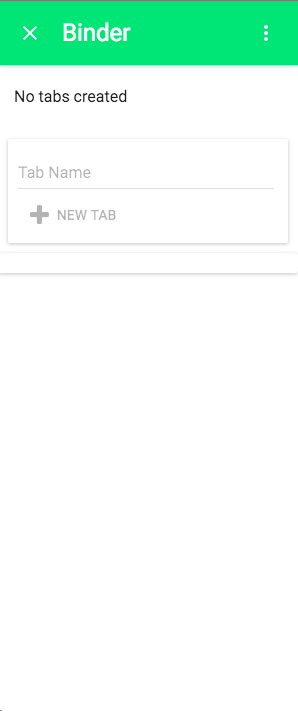
\includegraphics[width=.8\linewidth]{Figures/BinderEmpty.png}
  \caption{}
  \label{fig:binderempty}
\end{subfigure}%
\begin{subfigure}{.5\textwidth}
  \centering
  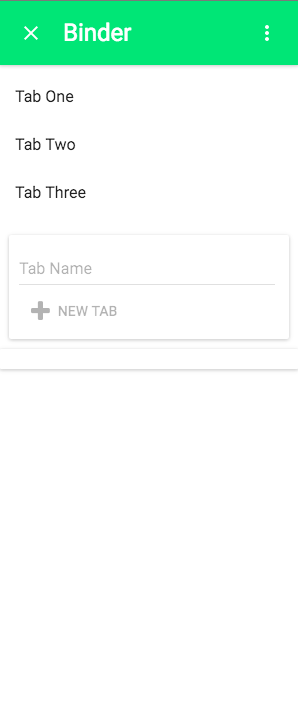
\includegraphics[width=.8\linewidth]{Figures/BinderFull.png}
  \caption{}
  \label{fig:binderfull}
\end{subfigure}
\caption{Binder, top level container for tabs. fig \ref{fig:binderempty} and \ref{fig:binderfull} show empty and full binders respectively}
\label{fig:binder}
\end{figure}

\begin{figure}
\begin{subfigure}{.5\textwidth}
  \centering
  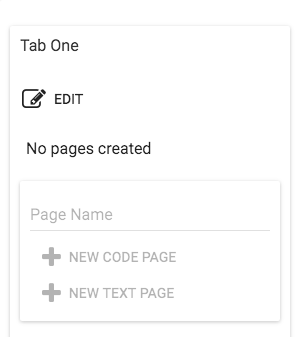
\includegraphics[width=.8\linewidth]{Figures/PagesEmpty.png}
  \caption{}
  \label{fig:pagesempty}
\end{subfigure}%
\begin{subfigure}{.5\textwidth}
  \centering
  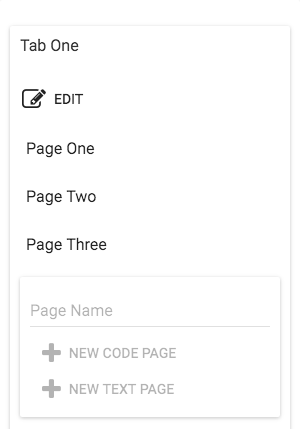
\includegraphics[width=.8\linewidth]{Figures/PagesFull.png}
  \caption{}
  \label{fig:pagesfull}
\end{subfigure}
\caption{Tabs, the second level container. fig \ref{fig:pagesempty} and
\ref{fig:pagesfull} show an empty and full tab respectively. This is shown
when a tab is selected, the pages are listed with the ability to edit the list,
and add new items.}
\label{fig:pages}
\end{figure}

Fig \ref{fig:binder} shows the implemented simple folder structure. The names
given to the levels are as follows: Binder, top level container. Tab, second
level container. Fig \ref{fig:pages} shows how the second level container is
displayed.

\section{Search capability in the system}\label{search-capability-in-the-system}

The requirements gathering process clearly identified in multiple places the
need for the system to provide a quick and simple search function.

There are multiple ways to provide search functionality within a document
management system, some of which are suitable for the application and some are
not. The below is a summary of a few of the options and an evaluation of each.

The search feature should take the users query and provide access to the
matching files in the system. This part of the searching experience will be the
same for all the discussed methods. However the parts that differ in the
compared methods are:
\begin{itemize}
  \item the format of the users query
  \item the searching method
  \item the time taken to perform the search
  \item the presentation of the results
\end{itemize}

\subsection{Simple text search / serial scanning}%
\label{simple-text-search-serial-scanning}

The simplest method for searching in a collection of documents is taking a
simple query from the user (the search term), and searches for the occurrences
of the term in each file. Each match results in an item in the result list
displaying the name of the file, and the position within the document.

For example:

\begin{alltt}
    search term: \emph{test}
    results:
    - File A, line 13, chars 34-38
      - ... the users will then report on \emph{test}ing ...
    - File A, line 13, chars 10-13
      - Chapter 2: \emph{Test}ing ...
\end{alltt}

This technique is simple and for small amounts of files and content is fast to
compute. However, due to the fact that the algorithm is loosely linear in the
number of files this technique would be impractical for large numbers of files.
This technique, called ``serial scanning''\footnote{%
\url{https://en.wikipedia.org/wiki/Full_text_search\#Indexing}%
has more details on this.}%
, is only typically used for smaller amounts of text due to this problem.

\blockquote{ However, when the number of documents to search is potentially
large, or the quantity of search queries to perform is substantial, the problem
of full-text search is often divided into two tasks: indexing and searching.
}\cite{wiki:full-text-search}

This technique that wikipedia refers to is discussed below.

\subsection{Full text index}\label{full-text-index}

When the simple method of searching through all the files becomes too slow, one
alternative is to create a concordance
\footnote{\url{https://en.wikipedia.org/wiki/Concordance_(publishing)} for more
information}. This is a table of words in a publication (here a note) and where
those words appear within the document. By using this concordance in place of
searching the text directly, the application is able to search a smaller amount
of data to find the results and hence speed up the search process.

This requires that there is a pre-processing step before a search can be
completed. This needs to be recalculated each time a user changes a
document so that all subsequent queries can find the new content.

This is the tradeoff with the more complex methods for searching. This method
requires the index to be built / rebuilt before any searching can take place.
However this can be done ``offline'' and cached for later use.

\subsection{Extraction of keywords}\label{extraction-of-keywords}

Another method of searching the documents is by analysis of keywords. Indexing a
select few words per note instead of all the words as in \ref{full-text-index}
means smaller indexes and faster searches.
Either a list of keywords is created and left static or, machine learning
algorithms can learn which words are important within the page and index only
those words.

This is however only applicable when the user's search terms can be limited as
such. This is because if the user searches for a word that is contained within a
file in the application, it will only be found if the word is in the keywords
list. In the case of a note taking application, a search method that can fail to
find a word that exists in the  document is of little use. However indexes of
the popular search terms can help to find preliminary results for a query, or
provide caches of common queries.


%\subsection{Edit distance}\label{edit-distance}

%\begin{quote}
%JP maybe discuss fuzzy search
%\end{quote}

\subsection{Reasons for selecting simple text
search}\label{reasons-for-selecting-simple-text-search}

The numerous ways to search the text within a collection of documents
each provide there own ways to provide the results. While many of the
different search methods are concerned with the performance of a search
and their accuracy in terms of the results, the most basic search
discussed the Simple text search \emph{link above section} as discussed
can offer the features needed by most users of the application.

There are many other features that can be added to the functionality
provided by the Simple text search \emph{link} however these can be
added as an extension to the program after the initial release.

\section{Type of user interface}\label{type-of-user-interface}

The different types of user interface that designers can choose from
when designing applications can be categorized into a few main
categories:

\begin{verbatim}
- Command line
- GUI / WIMPS
\end{verbatim}

For visualizing text, popular command line applications for editing text
like Vim or Emacs do exist however, the richer environment of a GUI
application is predominately preferred with its ability to customize
fonts and other such attributes of the layout and style. They also
provide a better experience for users with the use of menus etc. These
can provide a more simple to use application than an alternate command
line program with many shortcuts to memorize.

There are many different types of GUI application that can be built and
an important decision that needs to be made before selecting the layout
of the application is what platform to build the application on.

\subsection{Native solution for operating
system}\label{native-solution-for-operating-system}

The first platform option is developing a desktop first application
native in a selected operating system. This would require selecting one
of the native windowing API's for the operating system. Some of these
API's are cross platform enabled for example see
\href{http://www.qt.io/}{qt} for a popular choice. Some more polished
and more integrated with the selected operating system for example
Apple's own windowing API is
\href{https://en.wikipedia.org/wiki/Cocoa_(API)}{Cocoa}

The advantages of using the operating system's manufacturer built API is
one of support from the company and choice of open source vs
proprietary. As one of the requirements is that the system should be
accessible the proprietary method is not an option for a time
constrained development like this. In order to complete a cross platform
version using operating system specific (non cross platform) API's would
mean a rewrite of the GUI code for each operating system that was to be
supported. The advantages of using the operating system's manufacturer
built API is one of support from the company and choice of open source
vs proprietary. As one of the requirements is that the system should be
accessible the proprietary method is not an option for a time
constrained development like this. In order to complete a cross platform
version using operating system specific (non cross platform) API's would
mean a rewrite of the GUI code for each operating system that was to be
supported.

\subsection{Mobile solution for Android /
IOS}\label{mobile-solution-for-android-ios}

The production of a mobile application for either the Android or IOS
markets would be done with either two versions of the application as
discussed with the desktop versions above, or there are tools like
\href{https://www.xamarin.com/platform}{Xamarin}

\begin{verbatim}
"Deliver native Android, iOS, and Windows apps, using existing skills,
teams, and code."
*cite xamerin*
\end{verbatim}

This allows for applications to be built for a variety of mobile
platforms with a single code base in C\#. The ability to ``write once
run anywhere'' is a big selling point for Xamarin and others like it.
However it would still restrict users into using mobile only.

\subsection{Browser based solution}\label{browser-based-solution}

With modern advances in browser technology it has become more feasible
to create full desktop replacement applications as website-applications.
These websites are truly cross platform, they can be viewed on any
platform with access to a web browser. Desktop OS or mobile OS alike can
all use one of a multitude of recent browsers from many vendors. -
Chrome (Windows, Mac OSX, IOS, Android) - Safari (Mac OSX, IOS, Windows)
- Opera (Windows, Mac OSX, IOS \{opera-mini\}, Android \{opera-mini\}) -
Firefox (Windows, Mac OSX, IOS, Android)

There are many different libraries on offer to help develop applications
with javascript. However it is still possible to create more traditional
client-server applications and have just a simple lightweight javascript
free front end. These applications tend to be slower and more cumbersome
to use because of there need to communicate every action with a server
over http.

An alternative to the more traditional client-server architecture is the
now more popular single page javascript application. This merges the
lines between the user perceived differences of the desktop and browser
experience.

A single page javascript application is a single web page that functions
like a normal application. The application have all the features of a
desktop application, they can make use of windows, buttons, and
animations etc\ldots{}

External data is gathered in background http calls (called Ajax
requests) and does not necessitate a full page reload. The absence of
these full reloads and the flash of white as the page loads give the
user a much better experience.

\emph{cite}

Single Page Web Applications By Michael S. Mikowski and Josh C. Powell

\subsection{Reason for selecting
browser}\label{reason-for-selecting-browser}

For the application being built the choice of platform is between a
cross platform library for a native desktop application and a web based
solution. For reasons of experience with technology and programming
languages developing for the browser was selected as the platform.

The browser application will be accessible from any platform and device
and provides an easy way to update the application in the future.

There are many different libraries that can help when building a
javascript application in the browser. The libraries have some things in
common and other unique points that set them apart from each other. Most
of the libraries cover the standard principles of MVC ``Model View
Controller'' or some similar variant thereof. See
\href{https://en.wikipedia.org/wiki/List_of_JavaScript_libraries\#Web-application_related_.28MVC.2C_MVVM.29}{here}
for a community populated list on wikipedia.

\subsection{Javascript MVC library -
React.js}\label{javascript-mvc-library---react.js}

React.js is a fairly new open source library from facebook.

\begin{verbatim}
A JAVASCRIPT LIBRARY FOR BUILDING USER INTERFACES

*cite React.js website*
https://facebook.github.io/react/
\end{verbatim}

React.js brings the notions of pure functions to the problem of creating
and updating views. In React.js the headache of updating the view when
something happens in the application is handled automatically. This is
accomplished by having the view hierarchy be a result of applying a pure
function of the application state. This has the important consequence of
removing the need for the developer to tell the application how an
action should update the UI. The developer only needs to update the
state and React.js will work out what needs to change by calculating the
difference in the old and new view hierarchies.

\subsection{Future React Native}\label{future-react-native}

React.js has a new related project created by the same team called React
Native. React Native takes the principles of React.js and with slight
tweaks to the code the same code can run as a native application on both
IOS and Android.

This would provide a way to get the application onto mobile devices in a
native environment the users wouldn't even know that the application was
even running in the browser.

\section{Choice of interface - Notebook
metaphor}\label{choice-of-interface---notebook-metaphor}

The interface of any application need to be simple and easy to
understand. the more complicated the interface the more brainpower needs
to be dedicated to using it. The most successful user interfaces provide
simple intuitive ways for uses to do the actions they require.

\begin{verbatim}
Metaphors are the fundamental concepts, terms, and images
by which information is easily recognized, understood, and
remembered.
- Metaphor Design for User Interfaces, Marcus, Aaron
\end{verbatim}

\emph{cite} @inproceedings\{Marcus:1998:MDU:286498.286577, author =
\{Marcus, Aaron\}, title = \{Metaphor Design for User Interfaces\},
booktitle = \{CHI 98 Cconference Summary on Human Factors in Computing
Systems\}, series = \{CHI '98\}, year = \{1998\}, isbn =
\{1-58113-028-7\}, location = \{Los Angeles, California, USA\}, pages =
\{129--130\}, numpages = \{2\}, url =
\{http://doi.acm.org/10.1145/286498.286577\}, doi =
\{10.1145/286498.286577\}, acmid = \{286577\}, publisher = \{ACM\},
address = \{New York, NY, USA\}, keywords = \{Web, consumers, culture,
diversity, graphic design, icons, information design, metaphors,
multi-media, productivity tools, rhetoric, semantics, semi-otics,
symbols, user interfaces, visible language\}, \}

The metaphor chosen for the application is the notebook. A physical
notebook has pages, tabs etc\ldots{} These are easily understood by
anyone who knows what a notebook is. We can extend the notion of a
notebook with concepts from the wider world of books with indexes and
contents pages.

The application will take from this notion of the ``notebook metaphor''
and from there the application interface will be designed.

\emph{notebook image mapped to uml diagram of application}

\section{Detachment of the SQL interface through custom web
API}\label{detachment-of-the-sql-interface-through-custom-web-api}

Selecting the browser poses some specific problems for a SQL IDE. A SQL
IDE needs to have access to the SQL server in order to execute queries
and retrieve results. There is no support in any of the mainstream
browsers for direct integration with a SQL server database, although
they do have limited support \emph{cite web sql} for in browser
databases.

This therefore requires the production of some middleware to connect the
database to the application. The commonly used method for transferring
data in the browser is via a JSON web API. There are many methods for
connecting to a SQL server database however, the Microsoft documentation
\emph{cite} https://msdn.microsoft.com/en-us/library/ms162132.aspx
contains C\#, VB, C++ documentation and libraries for querying the
database. I have experience using the C\# conneciton methods before and
with this in mind the middleware was chosen to be a C\# website
providing a mapping from JSON to the database.

\emph{diagram of connection}

\chapter{Implementation}\label{implementation}

This chapter in this report will detail how the application was
implemented given the choices made in the Design chapter and the
requirements. The application was developed in the agile methodologies.
Quick and small iterations where a small part of the application will be
planned, implemented and tested. By ensuring the parts are kept to a
consistent small size, the development should be kept going at a
methodical pace.

As always with development projects involving code version control is an
important part of the development process. For this project git has been
used to keep track of the changes to the code. This provides many
benefits as can be seen in Version Control with Git%
\footnote{\url{https://goo.gl/WqK6f2}}.

Keeping the iterations small and using technologies like git allows for more
agile development. Being agile means reacting to complications with development
and delays that occur due to new languages and technologies will have less
impact on the development process.

With this in mind, the application was broken down into smaller parts
that fit together to form the application. The front end of the system
is the part the users will directly be interacting with. This would form
the bulk of the development however; the backend of the application is
the middleware component that will enable the javascript front end to
talk to the database.

\section{Middleware}\label{middleware}

The middleware was planned to be created first. It was a simple task and
was well defined. The requirements for this part of the application were
as follows:

\begin{itemize}
\tightlist
\item
  Allow the caller to create a connection to a database.

  \begin{itemize}
  \tightlist
  \item
    This will require the caller to pass connection parameters and in
    return they will receive some connection token to represent the
    connection.
  \end{itemize}
\item
  Allow the caller to execute queries against a connected database.

  \begin{itemize}
  \tightlist
  \item
    Given the connection token received in the above step and a query,
    the results of the query need to be sent back to the caller.
  \end{itemize}
\item
  Allow the caller to receive context data regarding a query.

  \begin{itemize}
  \tightlist
  \item
    Similar to executing a query, the application might need to receive
    details about the objects mentioned in the query. Each object
    mentioned in the query, table, view, function etc\ldots{} would be
    explained in the response.
  \end{itemize}
\end{itemize}

\subsection{Design the API}\label{design-the-api}

The communication to the database is provided by use of the
SqlConnection and SqlCommand classes provided by C\#. To execute a query
you must first create a SqlConnection class with the connection string.
A connection string is a textual detail of the parameters required to
connect to the database. This can contain many different types of
connection however the more usual address and username and password will
be used to connect to the database in the api.
\begin{listing}[ht]
\begin{minted}{csharp}
    public class ContextRequest
    {
        public string Database { get; set; }
        public string Server   { get; set; }
        public string Username { get; set; }
        public string Password { get; set; }
    }
\end{minted}
\end{listing}

The ContextRequest class provides the definition for the parameters for
the CreateExecutionContext when the /api/CreateExecutionContext method
received a http post the parameters are extracted from the body of the
post and a sql connection is created, opened and a token is returned to
the user.

From javascript there are many different ways in which you can do a HTTP post.
The library that is used in the application is called superagent
\footnote{\url{http://visionmedia.github.io/superagent/} has more details and
documentation} this provides a set of functions that manage HTTP posts. Here is
an example of how a HTTP post can be made to \emph{url} with parameters
\emph{params}. When the post has completed the callback function is called with
the response.

\begin{listing}[ht]
\begin{minted}{javascript}
  request
    .post(url)
    .send(params)
    .type('application/json')
    .accept('application/json')
    .end(newCallback(callback));
\end{minted}
\end{listing}

Here the response is the connection token. This token will be needed to
execute all further requests to this connection.

\section{Javascript application}\label{javascript-application}

The javascript application provides the user interface for the
application. It is written in javascript and runs in the browser in a
single web page. Requests to the SQL middleware API are made over HTTP
with the superagent package.

Applications built for browsers can have very large codebases, There are many
different problems that arrive from having a large code base and there are tools
available to help developers manage the applications. With standard javascript
there is currently no module system (although this may change
soon\cite{javascriptes6}) so when the application is separated into multiple
files these must be loaded in the browser before being used. This can become
difficult with many interdependent and third party modules.

There are ways to automate this process and automatically find all dependancies
and bundle them all into one file. This bundle file contains a compiled and
compressed version of all of the different modules. The browser can then load
this single file. This enables developers to separate the different parts of the application and not have to
put time into loading each manually.

\href{http://browserify.org/}{Browserify} is one such program. The tool can be
used from the command line to compile the application into a single javascript
file. The Browserify process can also be extended to optimize our javascript
code and also provide us with analysis to point out potential bugs and best
practices. These tools help to turn the javascript development process into
something similar to ahead-of-time compiled code like C\# and Java and C++. This
is needed for larger applications to be built in the browser\footnote{other
tools such as \url{https://en.wikipedia.org/wiki/Emscripten} could have been
used instead to transpile c++ or c into javascript }.

\subsection{React.js development}\label{react.js-development}

With React.js the UI is defined by React components. Each component can
be thought of as a new html element. They can have attributes defined:

\begin{listing}[ht]
  \begin{minted}{html}
    <NewElement attributeNo1="Ted" attributeNo2="123.4"/>
  \end{minted}
\end{listing}

And each component has a render function, this render function takes
each components internal state and produces more html for the page.


\begin{verbatim}

    var HelloMessage = React.createClass({
    render: function() {
      return <div>Hello {this.props.name}</div>;
    }
    });

    ReactDOM.render(<HelloMessage name="John" />, mountNode);

\end{verbatim}

In the above example the HelloMessage component is created. In this
simple component when it is used it outputs just a simple html DIV
element.

The use of React.Js in the project forces structure in the use of
components. The layout of the application is as follows:

\begin{verbatim}

   - controllers/
   - helpers/ 
   - stores/ 
   - ui/ 
   - app.js

\end{verbatim}

The application is created in the app.js and this then uses the
components in the UI folder to create the interface. The app.js file
completely separates the UI into the binder (the left hand side of the
interface) and the workspace (where pages are opened).

\subsection{Storage of data}\label{storage-of-data}

The application will store the data for the open notebook in the browser
until it is closed and saved to disk. The data in the browser will form
the state of the react components and any changes to this state will
cause React.js to re-draw the UI.

The pages are stored in the PageStore module. The tabs are stored in the
TabStore module and the workspace in the WorkspaceStore module. Each of
the stores contains the current state of the objects and components that
need to access data from them add listeners when created and receive
events when things change. This way we can separate the code that stores
the data and modifies it and the code that creates the UI. This
separation of concerns simplifies the details the developers needs to be
aware of when writing code.

\subsection{Data store interface}\label{data-store-interface}

The interface that the application uses to change the data in the store.
It is important that this interface is as simple to use as possible in
order to ensure that all the complicated logic to change the data is
completely within the store.

First the actions were planned out that the user might trigger.

\begin{verbatim}
    - Create new page 
    - Save page 
    - Delete page 
    - Create new tab 
    - Change search text
    - Connect / Execute query
\end{verbatim}

These actions form events. When these events are triggered, the data stores
update the internal state. The changes in the state then cascade down to the
components that depend on them and update the UI.

\subsection{Components}\label{components}

The application was split into small functional parts and a high level
design for the application was drawn out.

\todo{diagram, of interface ``boxes''}

The left side of the application is dedicated to the navigation
interface with tabs and pages displayed with buttons to create new and
remove old.

The workspace is a container for the open pages in the application each
page is a different component depending on what type the page is. For
example a search page renders a Search component and an index page
renders an Index component. This allows for easy addition of new window
types to the system as each is implemented in a separate file.

The initial design was implemented with the standard html entities ``li''
for list and ``button'' for actions. Later in the design process these
were replaced with components form a third party library of elements. The library
provides styled components that can be used in place of standard html. 
The styled components also follow the design specification called
``material design''.\footnote{\url{https://design.google.com/spec/} for more
information} This design specification defined rules for positioning, coloring
and other visual semantics that give the application a profesional feel and 
also giving the design consistency with other applications that also use 
this style.

Changing the visual design of the system proved to be a simple task, this is
mostly due to the choice of technology. Browserify and React.js both contributed
by allowing a third pary library\footnote{\url{http://www.material-ui.com/}} to 
be easily imported and replace the unstyled components.

\chapter{Results}\label{results}

  In this chapter the results of the project will be shown. Annotated screenshots
  of the application will be shown with details of the 
  features and any interaction between components. 

\section{Overview}
\begin{center}
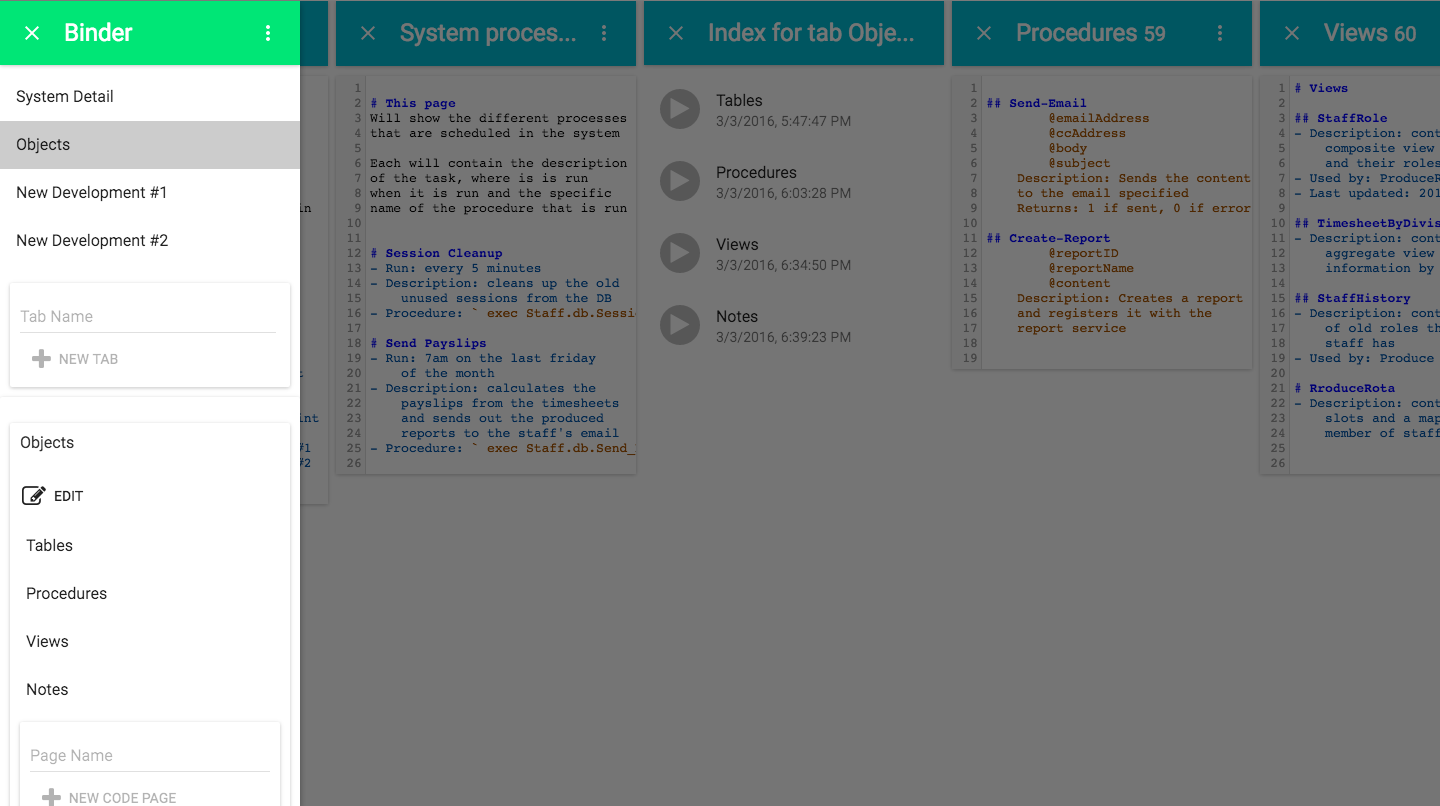
\includegraphics[width=0.8\textwidth]{Figures/Overview.png}
\end{center}

This screenshot shows an open notebook. The left hand side portion of the interface
shows the Binder the main navigational tool. Behind this is the workspace where the open pages
are displayed.

\section{Binder}
The Binder is a navigational interface. It provides a listing for all the files
in the system. The interface is separated into: the Menu bar, where the options are 
displayed, the Tabs list, and the Pages list.

The main purpose is to provide the user with the ability to explore the documents
and offer creation and deletion.

\subsection{Menu}

  \begin{center}
  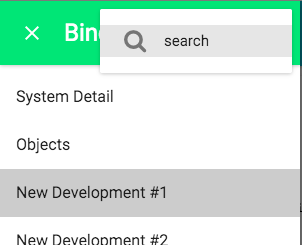
\includegraphics[width=0.3\textwidth]{Figures/Binder-Menu.png}
  \end{center}

  The Menu has only a single ``search'' option, this opens a new search window
  in the workspace.

\subsection{Tabs}

  \begin{center}
  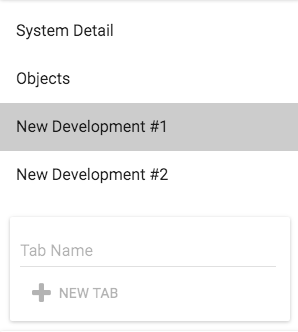
\includegraphics[width=0.3\textwidth]{Figures/Binder-Tabs.png}
  \end{center}

  The Tabs section of the Binder lists the Tabs in the project. Each tab in the
  list can be selected, showing the pages within in the Pages section below.

\subsection{Pages}

  \begin{center}
  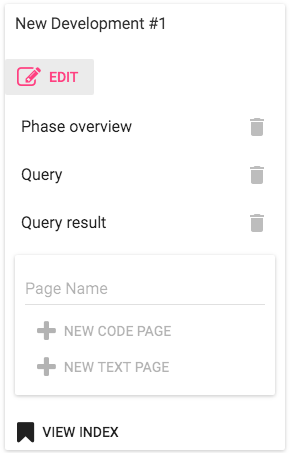
\includegraphics[width=0.3\textwidth]{Figures/Binder-Pages.png}
  \end{center}

  The Pages section is populated when a tab is selected. This section shows
  options for adding new code pages to contain SQL queries and text pages 
  to contain notes. The edit buttion can be selected to toggle edit mode. When
  in edit mode, each page has a delete icon that can be used to remove the page.

  The Index button at the bottom of the section when selected opens an Index page
  for the tab.

\section{Workspace}


  The Workspace is where pages appear when they are opened. The open pages are displayed
  horizontally with new pages opened on the right hand side of old ones. The user can have
  many window open at once.
\subsection{Search}

  \begin{center}
  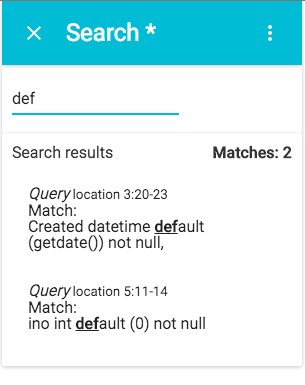
\includegraphics[width=0.3\textwidth]{Figures/Pages-Search.png}
  \end{center}

  The Search page has a single text box for the users search phrase. When the phrase 
  changes, the results in the bottom of the interface update to show the matches.

  Each match has the name of the page, location of the match and the excerpt from 
  the text.

\subsection{Index}

  \begin{center}
  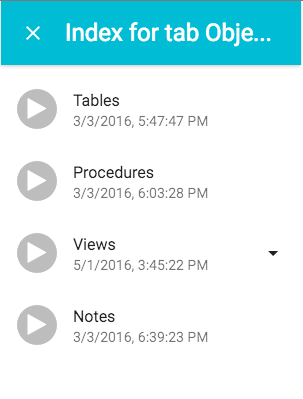
\includegraphics[width=0.3\textwidth]{Figures/Pages-Index.png}
  \end{center}

  The index shows the pages contained within a tab. Each page has the last
  modified date and time next to it from when it was last saved.  

  \begin{center}
  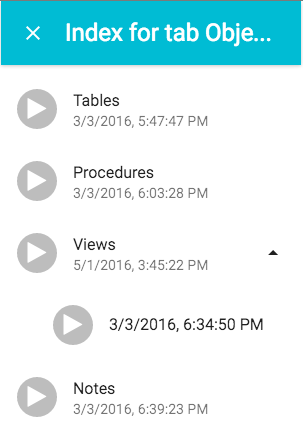
\includegraphics[width=0.3\textwidth]{Figures/Pages-Index2.png}
  \end{center}

  Here one of the pages shown in the index has a previous version stored.

\subsection{Note}

  \begin{center}
  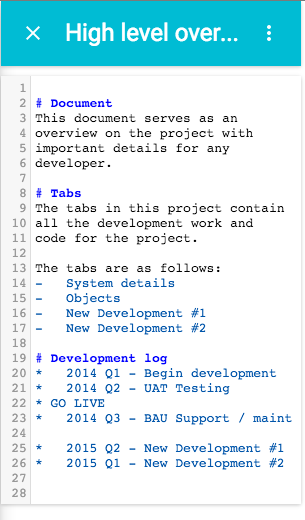
\includegraphics[width=0.3\textwidth]{Figures/Pages-Note.png}
  \end{center}

\subsection{Code}

  \begin{center}
  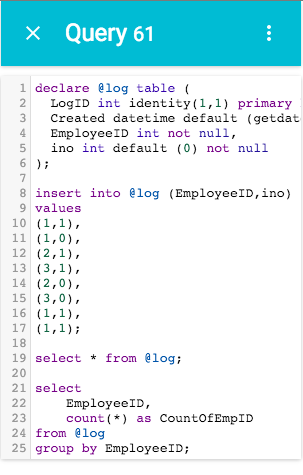
\includegraphics[width=0.3\textwidth]{Figures/Pages-Code.png}
  \end{center}

  \begin{center}
  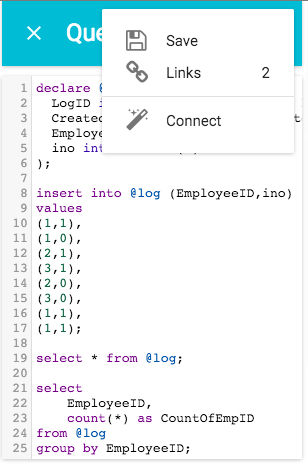
\includegraphics[width=0.3\textwidth]{Figures/Pages-Code-Menu.png}
  \end{center}

  The options available in the menu offer the ability to save, execute and reconnect the page to the database.

  \begin{center}
  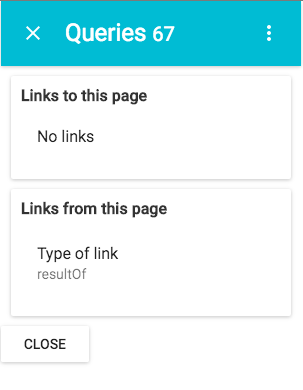
\includegraphics[width=0.3\textwidth]{Figures/Pages-Code-Links.png}
  \end{center}

  The links view, accessed from the menu shows the links this page has to the other items in the
  notebook. 

\subsection{Result}

  \begin{center}
  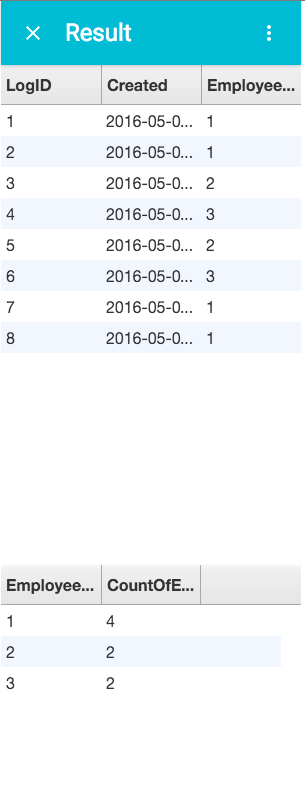
\includegraphics[width=0.3\textwidth]{Figures/Pages-Result.png}
  \end{center}

  The result from a query are shown in a result page. A scrolling table shows the rows in each result set.
  The menu offers the ability to save the result to the notebook for future use.



\chapter{Evaluation and Future
developments}\label{evaluation-and-future-developments}

\section{Testing the project}\label{testing-the-project}

Testing is an important part of developing an application. In order to achieve
its goals, the application must function correctly, with testing and
verification ensuring that each part of the system operates correctly.

The system was designed to be easily tested. The data store's interface
which provides the methods that the application uses was tested at the
beginning of each run of the application. The application would
initialise and then perform the testing procedure. The testing procedure
contained a simulation of a user performing some tasks, creating pages
and adding content etc..

After the system had finished running the user's commands the resulting
UI could be checked against the expected output and in this way
regression could be detected early. The JavaScript console also provides
an excellent way to monitor the application for errors at runtime and
debug to find their cause(s).

\section{Evaluation}\label{evaluation}

For the application to be successful the requirements and use cases need
to be evaluated against the application. The application will be
successful if each of the requirements are met and the use cases can be
shown to be completed by the users.

For my evaluation I presented the application to the users and asked them
to complete some simple tasks. The users had not seen the application
before and also had not seen any of the data stored before. This test
shows how easy the application is to learn and also provides
feedback on how real users interacted with the UI to find the
information stored in the system.

The testers were only told a bare minimum of what the application was
supposed to do. The application should allow for the organisation of
data and code for a SQL application.

Overall the testers were all able to find the various functions of
the application by navigating the familiar UI features like the burger
menu, ``X'' for closing windows. Finding the save options was
similarly found by them.

The tools for executing and saving the results from queries were also
quickly learned by the users. This feature requires the most ``clicks''
in the application and so could be viewed as the most complicated
feature however, the users rarely got lost and the actions flowed
naturally to the users.

The testers also made some comments on what features they would like to
see in the future for the application. These future features will be
discussed below.

\section{Future developments}\label{future-developments}

The application as it is can be used for daily work by SQL developers
and meets the requirements set out initially. However there are some
features that did not fit into the schedule of remaining time. These
features were not essential to completing a functional working
application however, they would make the application more useful.

\subsection{Multiple database
engines}\label{multiple-database-engines}

Currently the application only supports Microsoft SQL Server however
with the addition of more middle ware and a configurable settings window
the application could be made to talk to any database server.

This would enable the users to work on multiple systems across multiple
database providers. It would also open the application to the users that
solely use one of those databases.

\subsection{Query explanation}\label{query-explanation}

The middle ware supports a method to explain the objects referenced in a
query. This functionality could be used to provide code completions and
also more data when the objects are hovered over.

The meta-data could also be saved in the file when the page is saved.
This would then be available when the page was loaded. This could
provide extra context when looking into old queries.

\subsection{Different result formats}\label{different-result-formats}

The results from the queries are shown in a table. The results of
queries are just arrays of n-tuples but they could represent more
complex items like pi charts or folder hierarchies.

There could be some automatic classification of results to decide the
best way to display the results. Failing that, fall back onto manual
selection for the results presentation.

\subsection{Resizing windows}\label{resizable-windows}

The workspace shows the open pages and their controls. Currently the
application sizes these to have all the same width however, this might
not be optimal for some files. The developer has no control over how
they are presented. It would be a valuable feature of the system to be
able to reorder and resize the windows for each open page. This would
make the system more customizable for each user.

\chapter{Conclusion}\label{conclusion}

The application meets all the mandatory goals (11) set out in the use cases.
Out of the two optional requirements, only one was met by the application.
This is due to the lack of remaining development time. The
delays in the development of the features of the application were
partially due to lack of experience with the workflow and the associated
technologies.

The build process especially was time consuming to pick up. This was
partially due to the many options available. The lack of up to date
information is only apparent after a new build step is required. These
delays and set backs only affect the momentum of the
development at the beginning of the project and after the changes have
been implemented development speeds up.

The implementation of the application, after a change of method for
storing the application data, was extensible and offers a good platform
for new features to be developed. The code is of good quality with
good code separation. The separate modules have an average length of only 80
lines, this short average file size is a good indicator of good quality code

The users who have seen the application have also offered thoughts on
other uses of the application, most common is the view that the
application could be used as an education tool for new programmers to
teach the code and the concepts behind database design.

The designing of the final solution was mostly influenced by personal
issues identified from personal experience working on database projects.
A more structured exploration into issues and solutions with other
developers could have come up with some more diverse ideas. These same
users could have been consulted at various stages of the development and
provided feedback.

Overall the project was a success and the final application has exceeded
initial expectations of what could be accomplished in a third year project.


\medskip

\printbibliography

\end{document}
